\documentclass{article}
\usepackage[utf8]{inputenc}
\usepackage{hyperref}
\usepackage[left=20mm,top=20mm,right=20mm,bottom=20mm]{geometry}
\usepackage{etoolbox} %required for cover page
\usepackage{booktabs}
\usepackage[usestackEOL]{stackengine}
\usepackage[T1]{fontenc}
\usepackage[utf8]{inputenc}
\usepackage{bm}
\usepackage{graphicx}
\usepackage{subcaption}
\usepackage{amsmath}
\usepackage{amsfonts}
\usepackage{mathtools}
\usepackage{xcolor}
\usepackage{float}
\usepackage{hyperref}
\usepackage[capitalise]{cleveref}
\usepackage{enumitem,kantlipsum}
\usepackage{amssymb}
\usepackage[square,numbers,sort]{natbib}
\usepackage[ruled,vlined]{algorithm2e}
\usepackage{listings}
\usepackage{lscape}
\usepackage{longtable}
\usepackage{boldline}



\title{Laboratorio di Interazioni Fondamentali \\ Relazione esperienza 1}
\author{Irene Celestino}
\date{8/11/2022}

\begin{document}
\maketitle

\subsection{Conteggi e incertezze sui conteggi}
Le misure di efficienza si basano sui conteggi dei segnali in uscita dai discriminatori e dalle unità di coincidenza, quindi per prima cosa ho stimato l'incertezza nella misura dei conteggi. 
\\
La statistica dei conteggi per unità di tempo è una poissoniana, quindi potrebbe risultare ragionevole prendere come incertezza la radice quadrata del valore misurato, in quanto per le poissoniane la varianza è uguale alla media. 
\\
Tuttavia, ho ripetuto molte volte la misura dei conteggi per unità di tempo in singola e in doppia tenendo fisse le alimentazioni dei fotomoltiplicatori e ho notato che il range in cui variano le misure è inferiore alla radice del numero di conteggi. \\
A titolo di esempio, riporto in tabella \ref{errcont} diverse misure dei conteggi in singola (acquisite in un intervallo di 100 s) del fotomoltiplicatore PM7 alimentato sempre a 1740 V. 

\begin{table}[h!]
\centering
\begin{tabular}{|c|c|}
\hline
Conteggi per secondo cps & $\sigma =\sqrt{\text{cps}}$ \\ 
 \hline
\hline 
96.72 &  9.83 \\ 
\hline 
98.52 &  9.93 \\ 
\hline 
94.57 &  9.72 \\ 
\hline 
97.07 &  9.85 \\ 
\hline 
94.16 &  9.70 \\ 
\hline 
95.76 &  9.79 \\ 
\hline 
99.49 &  9.97 \\ 
\hline 
97.47 &  9.87 \\ 
\hline 
99.45 &  9.97 \\ 
\hline 
97.00 &  9.85 \\ 
\hline 
94.84 &  9.74 \\ 
\hline 
96.15 &  9.81 \\ 
\hline 
92.03 &  9.59 \\ 
\hline 
96.48 &  9.82 \\ 
\hline 
96.02 &  9.80 \\ 
\hline 
96.16 &  9.81 \\ 
\hline 
94.67 &  9.73 \\ 
\hline 
92.38 &  9.61 \\ 
\hline 
\end{tabular}
\caption{Fluttuazioni della misura dei conteggi per secondo in singola per PM7}\label{errcont}
\end{table}

Il valore medio dei conteggi per secondo è 96.05, con una media delle radici dei conteggi di 9.80. \\
Invece, l'errore massimo di queste misure, cioè $\frac{\text{max(cps) - min(cps)}}{2}$, è 3.73, inferiore all'errore stimato con la radice del numero di conteggi. Ancora di più è basso lo scarto quadratico medio, pari a 2.02.
\\
Per il fotomoltiplicatore PM4 (alimentato a 1670 V) si ottengono risultati analoghi: la media dei cps è 92.49, la media delle radici è 9.62, mentre l'errore massimo è 5.33 e lo scarto quadratico medio è 3.03.
\\
Dato però che per la maggior parte dei conteggi ho preso una sola misura una volta fissata l'alimentazione, considererò sempre come errore la radice del numero di conteggi per secondo, anche se questo valore può essere una sovrastima dell'intervallo in cui possono variare le misure dei conteggi. 
\newpage
\subsection{Conteggi delle coincidenze doppie, triple e dell'efficienza}

Per questa prima parte ho lavorato fissando le alimentazioni dei tre fotomoltiplicatori in modo da avere un rate di conteggi in singola di circa 100 cps, come indicato in sezione 3. In particolare, le alimentazioni soni 1740 V per PM7, 1685 V per PM5 e 1670 V per PM4.
\\
Ho poi misurato i conteggi delle coincidenze in doppia per ogni coppia di fotomoltiplicatorei e in tripla, ottenendo i risultati riportati in tabella \ref{tabdoppie}. Nell'ultima colonna è presente una prima stima dell'efficienza, calcolata come rapporto tra numero di coincidenze triple e numero di coincidenze doppie degli altri due fotomoltiplicatori.

\begin{table}[h!]
\centering
\begin{tabular}{|c|c|c|c|c|}
\hline
Fotomoltiplicatore &  Singola [cps] &  Coincidenza doppia [cps] & Coincidenza tripla [cps]  & Efficienza \\ 
\hline
\hline 
PM7 & $98.5 \pm 9.9$ & & &\\ 
PM5  & $123.9 \pm 11.1$ & $1\&3=7.37 \pm 2.71$  & $7.09 \pm 2.66$ & $\epsilon_2= 0.96 \pm 0.36$ \\ 
PM4  & $94.1 \pm 9.7$ & & &\\ 
\hline 
PM7 &  $100.1 \pm 10.0$ & & &\\ 
PM5  & $126.3 \pm 11.2$ & $1\&2 = 11.80 \pm 3.44$  & $7.90 \pm 2.81$ & $\epsilon_3= 0.67 \pm 0.23$\\ 
PM4 & $88.1 \pm 9.4$ & &  &\\ 
\hline 
PM7  & $94.2 \pm 9.7$ & & &\\ 
PM5  & $126.3 \pm 11.2$ & $2\& 3 = 14.98 \pm 3.87$  & $6.23 \pm 2.50$ & $\epsilon_1= 0.42 \pm 0.17$\\ 
PM4  & $87.0 \pm 9.3$ & & & \\ 
\hline
\end{tabular}
\caption{Conteggi in coincidenza doppia e tripla ad alimentazioni fissate}\label{tabdoppie}
\end{table}

\section{Efficienza dei fotomoltiplicatori al variare dell'alimentazione}

\subsection{Efficienza del secondo fotomoltiplicatore (PM5) al variare della sua alimentazione}
Per prima cosa, ho studiato l'andamento dell'efficienza del secondo fotomoltiplicatore (PM5) variando solo la sua tensione di alimentazione e tenendo fisse le altre due, a 1740 V per PM7 e 1670 V per PM4.
\\
L'efficienza di PM5 può essere stimata come $\epsilon_2 = \frac{n(1\&2\&3)}{n(1\&3)}$. \\ 
Per quanto riguarda le incertezze, dato che prendevo contemporaneamente le misure di $n(1\&2\&3)$ e di $n(1\&3)$, ho considerato i conteggi in doppia senza errore, in quanto ogni volta ridefiniscono il $100\%$ dei conteggi e non importa quanto il loro valore fluttui. 
Per questo motivo, ho considerato solo l'incertezza su $n(1\&2\&3)$, prendendo la radice del numero dei conteggi. \\
La misura dell'efficienza è data quindi in prima battuta, senza considerare le coincidenze accidentali, da: 
\begin{equation}
\epsilon_2 = \frac{n(1\&2\&3)}{n(1\&3)} \pm  \frac{\sqrt{n(1\&2\&3)}}{n(1\&3)}
\end{equation}

\subsubsection{Tabella con le misure per $\epsilon_2$}
Ho variato la tensione di alimentazione del secondo fotomoltiplicatore tra 1500 V e 1900 V e per ogni valore ho misurato per 100 s il numero di conteggi in singola dei tre fotomoltiplicatori, in coincidenza doppia $1\&3$ e in coincidenza tripla $1\&2\&3$.
\\
In tabella \ref{tabepsilon2} si possono vedere tutte le misure che ho preso con le relative incertezze. 
\\
Tutte le misure dell'efficienza di PM5 sono state riportate in figura \ref{fepsilon2}. 
\newpage

\begin{table}[H]
\centering
\begin{tabular}{|c|c|c|c|c|c|}
\hline
Fotomoltiplicatore & Alimentazione PM5 & Conteggi in singola [cps] & $1 \& 3$  [cps]&  $1\&2\& 3$ [cps]& $\epsilon_2$\\ 
 \hline
\hline 
PM7 & & $92.0 \pm 9.6$ & & & \\ 
PM5 & 1500 & $7.0 \pm 2.6$& $7.5 \pm 2.7$  & $1.7 \pm 1.3$ & $0.23 \pm 0.17$\\ 
PM4 & & $89.6 \pm 9.5$ & & & \\ 
\hline 
PM7 & & $96.0 \pm 9.8$ & & & \\ 
PM5 & 1520 & $9.6 \pm 3.1$& $6.7 \pm 2.6$  & $2.4 \pm 1.5$ & $0.36 \pm 0.23$\\ 
PM4 & & $89.8 \pm 9.5$ & & & \\ 
\hline 
PM7 & & $96.2 \pm 9.8$ & & & \\ 
PM5 & 1540 & $13.7 \pm 3.7$& $6.8 \pm 2.6$  & $3.4 \pm 1.8$ & $0.49 \pm 0.27$\\ 
PM4 & & $88.8 \pm 9.4$ & & & \\ 
\hline 
PM7 & & $94.8 \pm 9.7$ & & & \\ 
PM5 & 1550 & $16.3 \pm 4.0$& $6.4 \pm 2.5$  & $3.6 \pm 1.9$ & $0.57 \pm 0.30$\\ 
PM4 & & $91.4 \pm 9.6$ & & & \\ 
\hline 
PM7 & & $96.2 \pm 9.8$ & & & \\ 
PM5 & 1575 & $26.6 \pm 5.2$& $6.8 \pm 2.6$  & $4.9 \pm 2.2$ & $0.72 \pm 0.33$\\ 
PM4 & & $90.8 \pm 9.5$ & & & \\ 
\hline 
PM7 & & $97.0 \pm 9.8$ & & & \\ 
PM5 & 1600 & $39.9 \pm 6.3$& $7.1 \pm 2.7$  & $6.2 \pm 2.5$ & $0.88 \pm 0.35$\\ 
PM4 & & $92.4 \pm 9.6$ & & & \\ 
\hline 
PM7 & & $92.4 \pm 9.6$ & & & \\ 
PM5 & 1625 & $58.1 \pm 7.6$& $7.1 \pm 2.7$  & $6.6 \pm 2.6$ & $0.93 \pm 0.36$\\ 
PM4 & & $88.9 \pm 9.4$ & & & \\ 
\hline 
PM7 & & $94.7 \pm 9.7$ & & & \\ 
PM5 & 1650 & $82.1 \pm 9.1$& $6.8 \pm 2.6$  & $6.6 \pm 2.6$ & $0.96 \pm 0.37$\\ 
PM4 & & $89.0 \pm 9.4$ & & & \\ 
\hline 
PM7 & & $98.5 \pm 9.9$ & & & \\ 
PM5 & 1685 & $123.9 \pm 11.1$& $7.4 \pm 2.7$  & $7.1 \pm 2.7$ & $0.96 \pm 0.36$\\ 
PM4 & & $98.1 \pm 9.9$ & & & \\ 
\hline 
PM7 & & $94.6 \pm 9.7$ & & & \\ 
PM5 & 1695 & $140.4 \pm 11.8$& $7.2 \pm 2.7$  & $7.0 \pm 2.6$ & $0.97 \pm 0.37$\\ 
PM4 & & $94.6 \pm 9.7$ & & & \\ 
\hline 
PM7 & & $97.1 \pm 9.9$ & & & \\ 
PM5 & 1710 & $163.5 \pm 12.8$& $7.1 \pm 2.7$  & $6.9 \pm 2.6$ & $0.97 \pm 0.37$\\ 
PM4 & & $94.2 \pm 9.7$ & & & \\ 
\hline 
PM7 & & $95.8 \pm 9.8$ & & & \\ 
PM5 & 1730 & $204.7 \pm 14.3$& $6.9 \pm 2.6$  & $6.8 \pm 2.6$ & $0.99 \pm 0.38$\\ 
PM4 & & $93.9 \pm 9.7$ & & & \\ 
\hline 
PM7 & & $96.7 \pm 9.8$ & & & \\ 
PM5 & 1750 & $244.4 \pm 15.6$& $6.7 \pm 2.6$  & $6.7 \pm 2.6$ & $0.99 \pm 0.38$\\ 
PM4 & & $99.5 \pm 10.0$ & & & \\ 
\hline 
PM7 & & $94.2 \pm 9.7$ & & & \\ 
PM5 & 1780 & $368.0 \pm 19.2$& $7.0 \pm 2.6$  & $6.9 \pm 2.6$ & $0.98 \pm 0.37$\\ 
PM4 & & $93.7 \pm 9.7$ & & & \\ 
\hline 
PM7 & & $99.5 \pm 10.0$ & & & \\ 
PM5 & 1810 & $710.8 \pm 26.7$& $7.4 \pm 2.7$  & $7.3 \pm 2.7$ & $0.99 \pm 0.37$\\ 
PM4 & & $95.8 \pm 9.8$ & & & \\ 
\hline 
PM7 & & $97.5 \pm 9.9$ & & & \\ 
PM5 & 1850 & $1311.1 \pm 36.2$& $7.2 \pm 2.7$  & $7.2 \pm 2.7$ & $0.99 \pm 0.37$\\ 
PM4 & & $92.6 \pm 9.6$ & & & \\ 
\hline 
PM7 & & $99.5 \pm 10.0$ & & & \\ 
PM5 & 1870 & $1551.7 \pm 39.4$& $6.9 \pm 2.6$  & $6.8 \pm 2.6$ & $0.99 \pm 0.38$\\ 
PM4 & & $91.5 \pm 9.6$ & & & \\ 
\hline 
PM7 & & $96.5 \pm 9.8$ & & & \\ 
PM5 & 1900 & $1858.2 \pm 43.1$& $7.2 \pm 2.7$  & $7.1 \pm 2.7$ & $0.99 \pm 0.37$\\ 
PM4 & & $90.4 \pm 9.5$ & & & \\ 
\hline
\end{tabular}
\caption{Conteggi per la stima di $\epsilon_2$}\label{tabepsilon2}
\end{table}

\newpage

\subsubsection{Grafico di $\epsilon_2$ al variare dell'alimentazione di PM5}
In figura \ref{fepsilon2} sono riportate le misure dell'efficienza di PM5 al variare della sua alimentazione. 
\\
Si può vedere che la sua efficienza è molto alta (intorno al $98-99\%$) nel regime in cui è pienamente funzionante, ovvero oltre i 1600 V, mentre scendendo sotto questa tensione l'efficienza cala velocemente. \\
In particolare, la tensione di alimentazione per cui l'efficienza è dimezzata è 1540 V.

\begin{figure}[h!]
\begin{center}
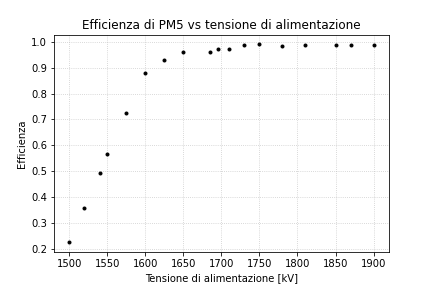
\includegraphics[scale=0.7]{Grafici/epsilon_vs_alimentazione_PM5.png}
\caption{Efficienza $\epsilon_2$ al variare della tensione di alimentazione del secondo fotomoltiplicatore PM5, mantenendo le altre due alimentazioni costanti} \label{fepsilon2}
\end{center}
\end{figure}

\subsubsection{Coincidenze accidentali}

Il numero di coincidenze doppie accidentali tra il primo e il terzo fotomoltiplicatore può essere stimato nel seguente modo. \\
Definiamo le seguenti quantità: 
\begin{itemize}
\item $R_1$ = numero di conteggi per secondo del primo fotomoltiplicatore
\item $R_3$ = numero di conteggi per secondo del terzo fotomoltiplicatore
\item $w_i$ = durata temporale del segnale in uscita dal discriminatore che va in ingresso all'unità di coincidenza (nel nostro caso vale 50 ns per entrambi i fotomoltiplicatori)
\item $w_{\text{min}}$ = tempo minimo per cui si devono sovrapporre due segnali in ingresso all'unità di coincidenza per avere in uscita un segnale diverso da zero (nel nostro caso vale circa 2 ns)
\item $\Delta t$ = durata dell'acquisizione
\end{itemize}
Una stima del numero di coincidenze accidentali è data da: 
\begin{equation}
n(1\&3)_{\text{acc}} = \Delta t \cdot R_1 \cdot R_3 \cdot (w_1+w_3-2w_{\text{min}}) \simeq 0.085
\end{equation}
Quindi il numero medio di coincidenze accidentali, 0.085, è molto minore rispetto al numero delle coincidenze doppie $1\&3$ misurate (in media circa 7), e si possono trascurare in questo caso le coincidenze accidentali. 
\newpage
\subsection{Efficienza del primo fotomoltiplicatore (PM7) al variare della sua alimentazione}
Analogamente, poi ho studiato l'andamento dell'efficienza del primo fotomoltiplicatore (PM7) variando solo la sua tensione di alimentazione e tenendo fisse le altre due, a 1685 V per PM5 e 1670 V per PM4.
\\
In tabella \ref{tabepsilon1} e in figura  \ref{fepsilon1}  si possono vedere le misure di efficienza, intesa come rapporto tra coincidenze triple e doppie, per il primo fotomoltiplicatore. L'andamento che si osserva è analogo a PM5, ma il valore massimo di $\epsilon_1$ è molto più basso, pari al $58\%$.\\
Questo si può spiegare con il fatto che, mentre se una particella che passa per il primo e il terzo scintillatore deve aver attraversato necessariamente il secondo, possono esserci benissimo particelle con traiettorie che intersecano solo il primo scintillatore. 

\begin{table}[H]
\centering
\begin{tabular}{|c|c|c|c|c|c|}
\hline
Fotomoltiplicatore & Alimentazione PM7 & Conteggi in singola [cps] & $2 \& 3$  [cps]&  $1\&2\& 3$ [cps]& $\epsilon_1$\\ 
 \hline
\hline 
PM7 & & $6.7 \pm 2.6$ &  & &\\ 
PM5 & 1670 & $125.0 \pm 11.2$ & $14.8 \pm 3.8$  & $1.7 \pm 1.3$ & $0.11 \pm 0.09$\\ 
PM4 & & $88.4 \pm 9.4$ &  & &\\ 
\hline 
PM7 & & $94.2 \pm 9.7$ &  & &\\ 
PM5 & 1740 & $126.3 \pm 11.2$ & $15.0 \pm 3.9$  & $6.2 \pm 2.5$ & $0.42 \pm 0.17$\\ 
PM4 & & $87.0 \pm 9.3$ &  & &\\ 
\hline 
PM7 & & $1039.0 \pm 32.2$ &  & &\\ 
PM5 & 1800 & $118.9 \pm 10.9$ & $14.4 \pm 3.8$  & $8.3 \pm 2.9$ & $0.58 \pm 0.20$\\ 
PM4 & & $81.8 \pm 9.0$ &  & &\\ 
\hline 
PM7 & & $800.5 \pm 28.3$ &  & &\\ 
PM5 & 1850 & $125.5 \pm 11.2$ & $14.5 \pm 3.8$  & $7.9 \pm 2.8$ & $0.54 \pm 0.19$\\ 
PM4 & & $87.1 \pm 9.3$ &  & &\\ 
\hline 
PM7 & & $27723.3 \pm 166.5$ &  & &\\ 
PM5 & 1900 & $124.2 \pm 11.1$ & $14.9 \pm 3.9$  & $7.7 \pm 2.8$ & $0.52 \pm 0.19$\\ 
PM4 & & $89.4 \pm 9.5$ &  & &\\ 
\hline
\end{tabular}
\caption{Conteggi per la stima di $\epsilon_1$}\label{tabepsilon1}
\end{table}

\begin{figure}[h!]
\begin{center}
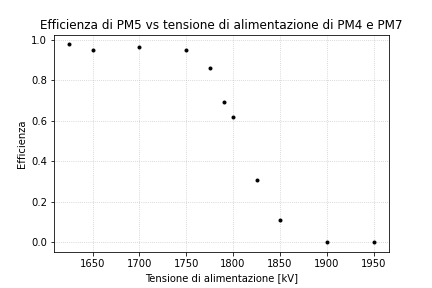
\includegraphics[scale=0.7]{Grafici/epsilon_vs_alimentazione_PM7.png}
\caption{Efficienza $\epsilon_1$ al variare della tensione di alimentazione del secondo fotomoltiplicatore PM7, mantenendo le altre due alimentazioni costanti} \label{fepsilon1}
\end{center}
\end{figure}

\newpage
\subsection{Efficienza del terzo fotomoltiplicatore (PM4) al variare della sua alimentazione}
Infine ho studiato l'andamento dell'efficienza del terzo fotomoltiplicatore (PM4) variando solo la sua tensione di alimentazione e tenendo fisse le altre due, a 1685 V per PM5 e 1740 V per PM7.
\\
In tabella \ref{tabepsilon3} e in figura  \ref{fepsilon3}  si possono vedere le misure di efficienza, intesa come rapporto tra coincidenze triple e doppie, per il terzo fotomoltiplicatore. L'andamento che si osserva è analogo a PM5 e PM7, ma il valore massimo di $\epsilon_3$, pari al $58\%$,è molto più basso rispetto a $\epsilon_2$, am più alto di $\epsilon_1$.\\
Per lo stesso motivo descritto nella sezione precedente ci aspettiamo che $\epsilon_3 < \epsilon_2$
\begin{table}[H]
\centering
\begin{tabular}{|c|c|c|c|c|c|}
\hline
Fotomoltiplicatore & Alimentazione PM4 & Conteggi in singola [cps] & $1 \& 2$  [cps]&  $1\&2\& 3$ [cps]& $\epsilon_3$\\ 
\hline
\hline 
PM7 & & $95.3 \pm 9.8$ &  & & \\ 
PM5 & 1550 & $126.1 \pm 11.2$ & $11.2 \pm 3.4$  & $0.5 \pm 0.7$& $0.04 \pm 0.06$\\ 
PM4 & & $2.3 \pm 1.5$ &  & &\\ 
\hline 
PM7 & & $96.5 \pm 9.8$ &  & & \\ 
PM5 & 1600 & $125.3 \pm 11.2$ & $11.7 \pm 3.4$  & $2.9 \pm 1.7$& $0.25 \pm 0.15$\\ 
PM4 & & $10.7 \pm 3.3$ &  & &\\ 
\hline 
PM7 & & $94.4 \pm 9.7$ &  & & \\ 
PM5 & 1640 & $127.1 \pm 11.3$ & $11.4 \pm 3.4$  & $5.6 \pm 2.4$& $0.49 \pm 0.21$\\ 
PM4 & & $37.3 \pm 6.1$ &  & &\\ 
\hline 
PM7 & & $100.1 \pm 10.0$ &  & & \\ 
PM5 & 1670 & $126.3 \pm 11.2$ & $11.8 \pm 3.4$  & $7.9 \pm 2.8$& $0.67 \pm 0.24$\\ 
PM4 & & $88.1 \pm 9.4$ &  & &\\ 
\hline 
PM7 & & $95.1 \pm 9.8$ &  & & \\ 
PM5 & 1700 & $125.7 \pm 11.2$ & $10.6 \pm 3.3$  & $7.4 \pm 2.7$& $0.70 \pm 0.26$\\ 
PM4 & & $166.5 \pm 12.9$ &  & &\\ 
\hline 
PM7 & & $99.3 \pm 10.0$ &  & & \\ 
PM5 & 1710 & $127.1 \pm 11.3$ & $9.3 \pm 3.0$  & $6.6 \pm 2.6$& $0.71 \pm 0.28$\\ 
PM4 & & $171.5 \pm 13.1$ &  & &\\ 
\hline 
PM7 & & $98.0 \pm 9.9$ &  & & \\ 
PM5 & 1750 & $126.9 \pm 11.3$ & $11.2 \pm 3.3$  & $8.3 \pm 2.9$& $0.74 \pm 0.26$\\ 
PM4 & & $828.5 \pm 28.8$ &  & &\\ 
\hline 
PM7 & & $94.8 \pm 9.7$ &  & & \\ 
PM5 & 1850 & $124.9 \pm 11.2$ & $10.4 \pm 3.2$  & $8.0 \pm 2.8$& $0.77 \pm 0.27$\\ 
PM4 & & $192482.3 \pm 438.7$ &  & &\\ 
\hline 
PM7 & & $95.7 \pm 9.8$ &  & & \\ 
PM5 & 1900 & $126.4 \pm 11.2$ & $11.6 \pm 3.4$  & $8.7 \pm 3.0$& $0.76 \pm 0.26$\\ 
PM4 & & $244425.2 \pm 494.4$ &  & &\\ 
\hline
\end{tabular}
\caption{Conteggi per la stima di $\epsilon_3$}\label{tabepsilon3}
\end{table}


\end{document}




